\chapter{Input Data}

In this chapter we will introduce our datasets that we use to evaluate recent Goce/Grace models in Sudan. 

\section{Astrogeodetic data}

In 1967 \cite{osman} during his studies at Cornell University has conducted a study to compute the geoid in Sudan. His data consists of 46 points for different locations in Sudan. Due to the lack of data from neighboring countries, and the huge gaps between measurements inside. He suggested to fill the gaps to have a reliable datum. For a detailed discussion about the attempts to compute datums for Sudan, reader is referred to \citep{ahmed_similar}. 

We have mentioned that \citet{osman} used an astro-geodetic observation, hence their datum is astro-geodetic datum. \citet{ahmed_msc} used gravity data to compute gravimetric datum for Sudan. The astro-geodetic datum, or \emph{geodetic datum} is a geoid computed by astronomically determined deflection of the vertical, while the gravimetric geoid is a geoid referred to the geocentric datum, hence the use of satellite data. A good discussion about the differences between the geoid types can be found in \cite{vanicek}. A sample of this data is provided in Table \ref{table:sudan_astro_data}. While the full data is provided in the appendix. The distribution of \citep{osman} work is introduced in Figure \ref{sudan_data}. 

\begin{table}[]
	\centering
	\caption{Astro-geodetic data for latitude longitude and geoid height}
	\label{table:sudan_astro_data}
		\begin{tabular}{@{}llll@{}}
			\toprule
			\emph{station} & $\phi \si{\degree}$  & $\lambda \si{\degree}$ & \emph{geoid height} $(m)$\\ \midrule
			
			zv & 22.1686 & 31.489 & 10\\
			12 & 20.1361 & 30.662 & 9.556\\
			28 & 18.4728 & 30.840 & 10.198\\
			43 & 17.0511 & 31.272 & 10.199\\
			53 & 14.4962 & 30.251 & 14.180\\
			70 & 13.8316 & 29.654 & 15.833\\
			76 & 13.2329 & 30.110 & 15.354\\
			79 &12.8660 & 29.956 & 15.647\\
			80 &12.7763 & 30.853 & 14.453\\
			85 &11.6038 & 30.411 & 15.387\\ \bottomrule
			
		\end{tabular}
\end{table}


\begin{figure}[t]
	\caption{Distribution of \citep{osman} points in Sudan. It is clear the huge gap that \citet{osman} suggested to be filled}
	\label{sudan_data}
	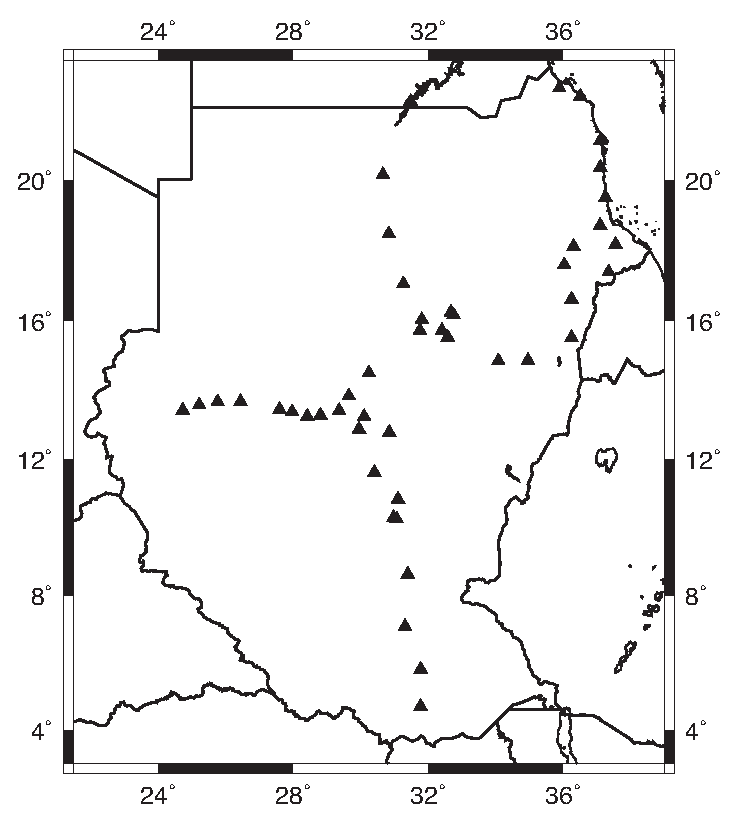
\includegraphics{Figures/points_dist.eps}
	\centering
\end{figure}


\section{GPS/Leveling Data}

GPS/leveling data are used to evaluate GGMs results by deriving the geoid height from them. The data were collected over Khartoum area. \\
GPS/Leveling data are two separate heights systems (orthometric and ellipsoidal height) for the same points (in terms of latitude and longitude). GPS data is ellipsoidal height data that is computed by means of GPS/GNSS systems. Leveling data on the other hand, is the orthometric height that is computed using spirit leveling. The geoid height can then be computed using Eq. \eqref{geoid_from_orthometric}

\begin{equation}
\label{eqn:geoid_from_orthometric}
N = h - H
\end{equation}

The GPS measurements were performed using dual frequency GPS receivers LEICA 1200, LEICA RS500 and Trimple 5700, and choke rings antennas ASH701945E\_M from Ashtech, LEICA AT504  used from \citet{ahmed_msc} work. The accuracy in leveling data is a bit problem because some of them were taken from a geodetic network of $3^{rd}$ order, which drastically affect our evaluations. The distribution of GPS/leveling results are shown in Figure \ref{fig:gps_khartoum}.

\begin{figure}[t]
	\caption{Distribution of GPS/leveling data over Khartoum}
	\label{sudan_data}
	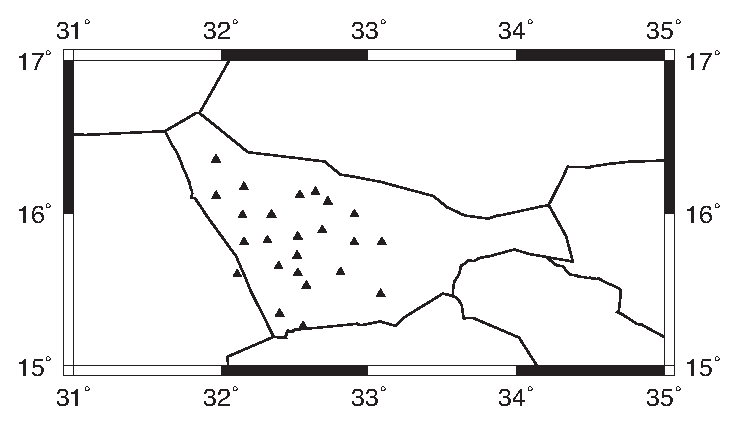
\includegraphics{Figures/points_dist_krt}
	\centering
\end{figure}


\begin{table}[]
	\centering
	\caption{GPS/Leveling data for Khartoum area}
	\label{gps_leveling}
		\begin{tabular}{@{}llll@{}}
			\toprule
			\emph{id} & $\phi \si{\degree}$  & $\lambda \si{\degree}$ & \emph{geoid height} $(m)$ \\ \midrule
			1 & 16.1719143 & 32.15278395 & 3.573 \\
			2 & 15.822078561111 & 32.312747819444 & 2.998\\
			3 & 15.889747230556 & 32.683920419444 & 3.619\\
			4 & 16.076534180556 & 32.721614461111 & 3.119\\
			5 & 15.810990861111 & 33.086944869444 & 2.175\\
			6 & 15.809063111111 & 32.899570888889 & 2.285\\
			7 & 15.613491838889 & 32.808035077778 & 2.02\\
			8 & 16.351884494444 & 31.964771408333 & 4.174\\
			9 & 15.847591619444 & 32.517391980556 & 3.078\\
			10 &16.118530788889 & 32.531269330556 & 2.263\\
			11 &15.99188345 & 32.3404394 & 3.21\\
			12 &15.810295125 & 32.154373358333 & 3.21\\
			13 &16.11349295 & 31.965449913889 & 3.197\\
			14 & 15.992628230556 & 32.9012736 & 3.254\\
			15 & 15.987956075 & 32.144070430556 & 3.447\\
			16 & 15.469951816667 & 33.079683027778 & 2.297\\
			17 & 15.651378211111 & 32.388177761111 & 2.81\\
			18 & 15.721159511111 & 32.514142069444 & 2.655\\
			19 & 16.139034477778 & 32.637590772222 & 2.4199\\
			20 & 15.607008355556 & 32.518298555556 & 2.6729\\
			21 & 15.599259138889 & 32.107760216667 & 2.5378\\
			22 & 15.524018605556 & 32.576891125 & 2.5993\\
			23 & 15.258628422222 & 32.554645944444 & 2.2311\\
			24 & 15.340130033333 & 32.394058058333 & 2.6918\\ \bottomrule
			

		\end{tabular}
\end{table}


\section{Global Geopotential Models}

A global Geopotential Model is a mathematical function approximates the real gravity potential of the Earth. From such an approximation, all related gravity field functionals can be computed (e.g., gravity potential, gravity vector). However, other gravity field functionals e.g., \textit{geoid height, gravity anomaly and gravity disturbance, and the second radial derivative} cannot be computed without a defined reference system (Geodetic Reference System 1980). As the centrifugal part can be modeled easily and accurately. It is usually beneficial to select a global geopotential model (and degree) that is best fit to the local gravity field as base for a regional gravimetric model. This will reduce the error by Stokes' formula by reducing the amount of the geoid contribution to the total error.

\subsection{Satellite-only models} they are derived solely from the analysis of the satellite orbit. They use laser and Doppler measurements to track the satellites \cite{goce_sp123} Historically, these models were known to have a low precision due to

\begin{enumerate}
	\item the inability to track complete satellite orbits using ground-based stations
	\item imprecise modeling of atmospheric drag attraction
	\item the incomplete sampling of the global gravity due to the limited number of satellites
\end{enumerate}
 
 
 These issues were fixed by the new dedicated satellite missions in the earlier 2000s \cite{rummel}. In our study, we used two satellite-only models ITU\_GCC16 and ITU\_GRACE16 of 280, 180 degree and order respectively. 
 
 \subsection{Combined Models}
 
 These models are combined from different source. A GGM is combined with land and shiptrack
 gravity observations, and marine gravity anomalies \citet{amos}. It is often that combined models have higher degrees than satellite-only models. Even with the added source of e.g., terrestrial data, combined models are also limited in their precision because of their use of satellite-only models. In our study we have tested three different combined models namely EGM2008, EIGEN-6C4 (2014), and GECO (2015). They are all up to degree 2190, and we tested them up-to their maximum degree. One source of error caused by the combination of different regional (local) datums and the offset between them. \citet{heck} reported that the magnitude of errors due to the inconsistency of regional datums with global datum is underestimated. The source of error was due to the simplified free-air reduction procedure and of different kinds of height system. \citet{heck} in their work have show that the corresponding systematic errors in gravity anomalies are maximum in mid-latitudes. The error due to datums inconsistency is a systematic error.
 
 
 \subsection{Tailored Models}
 A combination of the aforementioned models designed (tailored) for a specific area. That actually against the term global in GGM. None of these models were tested in our experiments.
 
 
 \subsection{Difficulties in modeling the Earth from the space}\label{fundamental_satellite_problem}
 
 \citep{rummel} in their work reported that there are two problems in efficiently model the Earth using satellite observations. In particular they report that 1) satellites can be tracked from the ground only over short intervals
 and, as a consequence, the gravity signal ‘printed onto the orbit’ can only be extracted where
 it produces an orbit signal of large size such as at or close to orbit resonances, and 2) satellite motion is not determined by gravitation alone but disturbed by several types of surface forces of non-gravitational origin. The main objectives of the new satellite missions is to tackle these two fundamental problems.
 \section{New Satellite Missions}
 
 Because of the mentioned limitations of satellite missions, new dedicated satellite missions was launched in early 2000s to tackle those problems. There are three satellite missions launched for that purpose
 \subsection{CHAMP}
 {CHAMP} \textbf{CHA}llenging \textbf{M}inisatellite \textbf{P}ayload is a German small satellite mission for geoscientific and atmospheric research and applications, managed by GFZ. The orbit of CHAMP is almost circular (inclination 87\si{degree}) which gives it an advantage of getting homogeneous and complete global coverage. With an altitude of 454 km, it guarantees that the satellite can work in severe atmospheric conditions. It also has a direct on-board measurement to account for the non-gravitational orbit perturbations. . CHAMP uses satellite-to-satellite tracking working on high-to-low mode, i.e., GNSS satellites are tracking the spaceship position, and it uses an accelerometer to compute the geoid functionals (cf. \cite{luhr} for detailed discussions about CHAMP mission). 
 \\
 Clearly, the aforementioned issues with previous satellite mission was resolved in the new dedicated satellite mission. A detailed description of CHAMP, and other new satellite missions e.g., GOCE and GRACE will be presented in Table \ref{table:dedicate_satellite_missions}. 
 
 \subsection{GRACE}
 \textbf{G}ravity \textbf{R}ecovery and \textbf{C}limate \textbf{E}xperiment is the second satellite mission that was launched on March 2002. GRACE consists of two identical satellites separated by 220 km from each others, and at 500 km above the Earth surface. Unlike CHAMP, GRACE is uses satelite-to-satellite tracking to precise position determination, but it uses low-low mode to compute the gravity functionals i.e., the gravity is measured by the change of the distance between the twin satellites. Areas of slightly stronger gravity (greater masses) will affect the leading satellite first. An accelerometer will be used to measure the non-gravitational acceleration--common errors due to atmospheric attraction--such that only the accelerations caused by the gravity are measured. 
 \\
 It is common to find a model with data from different satellite mission--each one of them contribute to specific range of spherical harmonics degrees.
 
 \subsection{GOCE}
 The last mission in the new gravity measurement satellites era is GOCE. \textbf{G}ravity Field and Steady-State \textbf{O}cean \textbf{C}irculation \textbf{E}xplorer. It is specifically designed for the determination of the stationary gravity field – geoid and gravity anomalies – to high accuracy and spatial resolution \cite{rummel}. As reported by \citep(rummer), GOCE is the only satellite mission that was able to solve the problem of gravity observations from satellites that was introduced in Section \ref{fundamental_satellite_problem}. In summary, GOCE has tackled the classic problems of using satellite to compute the gravity as follow
 
 \begin{enumerate}
 	\item Uninterrupted tracking in three spatial dimensions
 	\item Measurement or compensation of the effect of non-gravitational forces
 	\item Orbit altitude as low as possible
 \end{enumerate}


 \section{Our models}
 For our study we have tested five models. Two of them are satellite-only models (ITU\_GCC16, and ITU\_GRACE16), three are combined models (EGM2008, EIGEN-6C4, and GECO). The choice of these models are based on their release date. The choice of the number of models is totally arbitrary.
 
 \begin{enumerate}
 	\item {ITU\_GCC16}. It was released on 2016 with degree and order up-to 280. A detail description about the mission can be found \href{http://www.geo.itu.edu.tr/gravity/ITU\_GGC16.html}{here}
 	
 	
 	\item {ITU\_GRACE16}. It was also released on 2016, with degree and order of 180. You can check their \href{http://www.geo.itu.edu.tr/gravity/ITU\_GRACE16.html}{website}
 	
 	
 	
 	\item{EGM2008}. The popular new version of EGM series, the previous ones were EGM84 and EGM96. We use this one for up-to degree of 2190. Released on 2008. For interested readers you can check their online website at \href{http://earth-info.nima.mil/GandG/wgs84/gravitymod/egm2008/index.html}{EGM2008}
 	\item {EIGEN-6C4}. Composed of data from different EIGEN series missions, in particular it uses data from EIGEN*‐6C, EIGEN‐6C2, and EIGEN‐6C3. It was released on 2014, and it is the last mission of EIGEN series. The model is up-to to degree and order of 2190. More details about the model can be found \href{http://icgem.gfz-potsdam.de/ICGEM/documents/Foerste-et-al-EIGEN-6C4.pdf}{here}
 	
 	\item {GECO}. It was released 2015, and it is the latest models of high o/d models (those above 2190 d/o). It combined data from GOCE mission as well as EGM2008. No available details about GECO model from ICGEM official website (at the time of writing this)
 	
 \end{enumerate}
 
 
 \section{An overview about this chapter}
 
 In this chapter we have introduced the new method of computing the geoid, or more generally measuring the surface of the Earth. While in the classic conservative approach to problems of physical geodesy as described by \cite{hoffmann}. The advantage of this approach is that the geoid as a reference surface has a very simple definition in terms of the physically meaningful and geodetically important, Potential $V$. The disadvantage, however, is that the potential $V$ inside the earth depends on the  density $\varrho$ because of the Poisson's equation Eq. \eqref{eqn:poisson}. 
 \begin{equation}
 \label{eqn:poisson}
	 \triangle W = - 4 \pi G \varrho
 \end{equation} 
 
 The mathematical aspects of GGM are reserved for the next chapter. It is clearly impossible that we cannot measure the density at each point in the earth, hence there should be some approximations. The other, or the modern approach is what proposed by Molodensky in 1945. He was able to show that the physical surface of the earth can be determined from geodetic measurements alone, without the need of the density of earth's crust. That means the concept of the geoid should be abandoned. This disadvantage is that the concept of the reference surface--which was easily defined by the geoid--will be more abstract, and the mathematical method will be more difficult.
 \\
 The development of satellite missions (that uses Molodensky's theory) was going such that with every new model there is a possible increase in degrees, and hence the accuracy. Table \ref{table:satellite_evolution} summarizes the major technical details regarding the new dedicated satellite missions. Table \ref{table:ggm_models} summarizes the models that were used in our study. 
 
 \begin{table}[]
 	\centering
 	\caption{Comparsion of new dedicated satellite missions}
 	\label{table:satellite_missions}
 	\begin{tabular}{@{}llll@{}}
 		\toprule
 		\emph{mission} & \emph{inclination angle \si{\degree}} & \emph{altitude (km)} \emph{release date} & status\\ \midrule
 		
 		CHAMP & 87.2777 & 454 & stopped-2010 \\
 		GRACE & 89 & 500 & still operating\\
 		GOCE & 96.7 & 268& still operating\\ \bottomrule
 		
 	\end{tabular}
 \end{table}
 
 
 \begin{table}[]
 	\centering
 	\caption{Breakthrough in satellite observations}
 	\label{table:satellite_evolution}
 	\begin{tabular}{@{}llll@{}}
 		\toprule
 		\emph{Mission} & \emph{Technology}  & mode & \emph{missions}\\ \midrule
 		SST-hl & Accelerometer & high-low & CHAMP \\
 		SST-ll & inter-satellite link & low-low& GRACE\\
 		SST-ll & Gradiometer & low-low & GOCE\\\bottomrule
 		
 	\end{tabular}
 \end{table}
 
 \begin{table}[]
 	\centering
 	\caption{Summary of GGM that were used in our study}
 	\label{table:ggm_models}
 	\begin{tabular}{@{}llll@{}}
 		\toprule
 		\emph{Model Name} & Type  & Max Degree \si{\degree} & \emph{Tested models} $(m)$\\ \midrule
 		ITU\_GGC16 & satellite-only & 280 & 270 \\
 		ITU\_GRACE16 & satellite-only & 180 & 170\\
 		EGM2008 & combined & 2190 & 500\\
 		EIGEN-6C4 & satellite-only & 2190 & 200\\
 		GECO & combined & 2190 & 500\\ 
 \bottomrule
 		
 	\end{tabular}
 \end{table}
 

